\documentclass[aspectratio=169,11pt]{beamer}

\usepackage[T1]{fontenc}
\usepackage[utf8]{inputenc}
\usepackage[magyar]{babel}
\usepackage{amsmath,amssymb,booktabs,graphicx,array,tikz}
\newcolumntype{L}[1]{>{\raggedright\arraybackslash}p{#1}}
\usetikzlibrary{arrows.meta,positioning,calc,fit,backgrounds,shapes.geometric,babel}

\usepackage{lmodern}
\usefonttheme{professionalfonts}
\usetheme{Madrid}
\definecolor{tdkblue}{RGB}{23,55,94}
\definecolor{priceblue}{HTML}{265D91}
\definecolor{shortteal}{HTML}{096C65}
\definecolor{gprpurple}{HTML}{674C8B}
\definecolor{eventochre}{HTML}{895810}
\definecolor{actualgreen}{HTML}{276444}
\definecolor{lossred}{HTML}{A23B32}
% Vízszintes, 100%-ra kiegészülő sáv: y, felirat, győzelem, döntetlen, vereség (%)
\newcommand{\qmbar}[5]{%
  \fill[actualgreen] (0,#1) rectangle (#3,#1+3.2);
  \fill[black!22] (#3,#1) rectangle (#3+#4,#1+3.2);
  \fill[lossred] (#3+#4,#1) rectangle (100,#1+3.2);
  \node[anchor=east, font=\tiny, text=black!60] at (-1,#1+1.6) {#2};
  \ifdim #3pt>12pt \node[text=white, font=\tiny\bfseries] at (#3/2,#1+1.6) {#3\,\%};\fi
  \ifdim #4pt>12pt \node[text=black!75, font=\tiny\bfseries] at (#3+#4/2,#1+1.6) {#4\,\%};\fi
  \ifdim #5pt>12pt \node[text=white, font=\tiny\bfseries] at (#3+#4+#5/2,#1+1.6) {#5\,\%};\fi
}
\setbeamercolor{structure}{fg=tdkblue}
\setbeamertemplate{navigation symbols}{}
\setbeamersize{text margin left=0.8cm,text margin right=0.8cm}
\setbeamerfont{frametitle}{size=\large}
\setbeamerfont{block title}{size=\normalsize}

\title[QuantiMate]{Tőzsdei prediktív folyamatok és algoritmikus\\döntéstámogató rendszerek kvantitatív modellezése}
\author{Csizmi}
\institute[EKKE]{Eszterházy Károly Katolikus Egyetem}
\date[]{2026.11.25.}

\begin{document}

% =====================================================================
% Időterv: 12 tartalmi dia + címdia, összesen 13:00. Tartalék: 2 dia.
% =====================================================================

% 1 | 0:00--0:20
\section{Bevezetés}
\begin{frame}
  \titlepage
\end{frame}

% 2 | 0:20--1:10
\begin{frame}{Kutatási kérdés}
  \begin{block}{Kérdés}
    Előre jelezhető-e az NVIDIA záróára és ingadozása 1, 5 és 21
    kereskedési napra pontosabban, mint modell nélküli referenciával,
    ha a túlillesztést szigorúan kizárjuk?
  \end{block}
  \medskip
  \textbf{Saját munka a QuantiMate rendszerben}
  \begin{itemize}
    \item Nyolc adatforrás időhelyes (point-in-time) illesztése.
    \item Két modellváltozat (V8, V8.5) közös kísérleti motoron.
    \item Kétlépcsős kiválasztási kapu és 18\,000 ismétléses kísérlet
          tervezése, futtatása.
  \end{itemize}
  % Referencia: árnál az utolsó záróár, ingadozásnál az EWMA-variancia.
\end{frame}

% 3 | 1:10--2:00
\section{Adatok és felépítés}
\begin{frame}{Adatok és időbeli illesztés}
  \centering\small
  \renewcommand{\arraystretch}{1.2}
  \begin{tabular}{@{}L{.2\linewidth}L{.47\linewidth}L{.27\linewidth}@{}}
    \toprule
    \textbf{Forrás} & \textbf{Adat} & \textbf{Mikortól használható}\\
    \midrule
    Yahoo Finance & napi árak: NVDA, SPY, QQQ, AMD, SMH, VIX, VXN, TNX & a nap zárásakor\\
    SEC EDGAR & gyorsjelentések, bennfentes ügyletek & következő kereskedési nap\\
    FINRA & shortállomány / napi shortforgalom & +9 munkanap / +1 nap\\
    Caldara--Iacoviello & geopolitikai kockázati index (GPR) & +2 nap\\
    FRED & kereskedelempolitikai bizonytalanság (EPU) & hónap vége +7 nap\\
    \bottomrule
  \end{tabular}
  \par\medskip\raggedright
  \begin{block}{Elv}
    A lezárás napján csak az akkor már nyilvános érték kerülhet a modellbe.
    Az adatok befagyasztott, SHA-256 ujjlenyomattal védett pillanatképből
    jönnek; futás közben nincs internet.
  \end{block}
  % Árak 2001-től; a tanításhoz a lezárás előtti 10 év kell.
\end{frame}

% 4 | 2:00--2:50
\begin{frame}{Két változat, közös motor}
  \centering\small
  \renewcommand{\arraystretch}{1.25}
  \begin{tabular}{@{}L{.22\linewidth}L{.34\linewidth}L{.34\linewidth}@{}}
    \toprule
    & \textbf{V8: több adatfajta} & \textbf{V8.5: több minta}\\
    \midrule
    Kiegészítő adatok & gyorsjelentés, insider, short, intraday, GPR, EPU & gyorsjelentés, insider, short\\
    Plusz változat & minden réteg együtt & 40 részvény közös tanítása (pooled)\\
    Hangolás & 2 rögzített beállítás & + 30 beállítás keresése PBO-fékkel\\
    Modell, kiválasztás & \multicolumn{2}{l}{LightGBM + HMM-rezsimek; azonos kétlépcsős kapu}\\
    \bottomrule
  \end{tabular}
  \par\bigskip\raggedright
  \textbf{Kísérlet:} 2 verzió $\times$ 2 cél (ár, ingadozás) $\times$ 3 táv
  (1, 5, 21 nap) $\times$ 30 dátumpár (2021--2025) $\times$ 50 seed
  $=$ \textbf{18\,000 futás}.
  % A két verzió ugyanabból az adatból, ugyanazzal a kóddal fut.
\end{frame}

% 5 | 2:50--4:00
\begin{frame}{Egy futás menete}
  \centering
  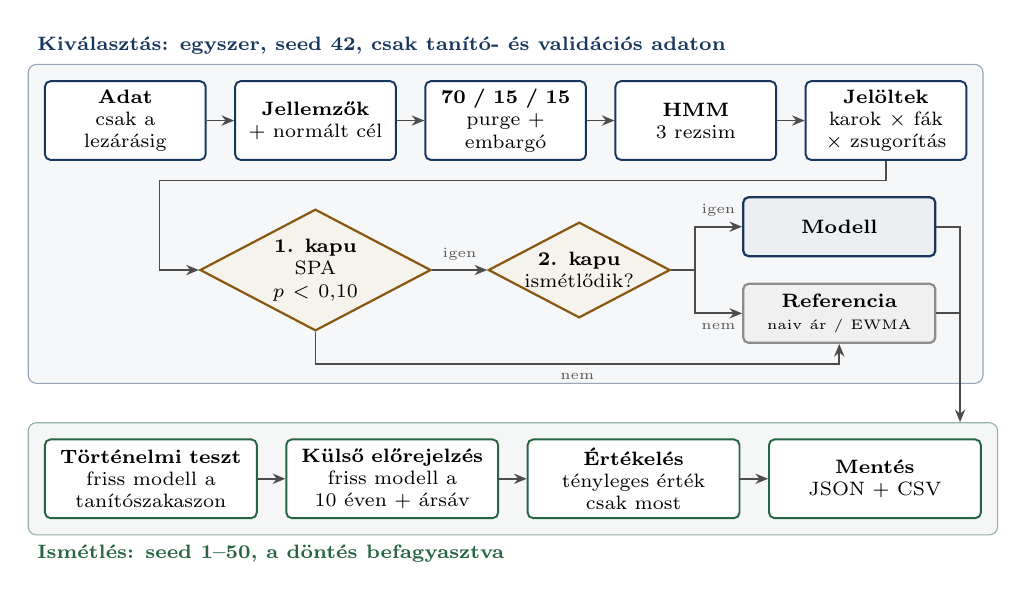
\begin{tikzpicture}[
    font=\scriptsize,
    st/.style={rectangle, rounded corners=2pt, line width=.7pt, draw=tdkblue,
      fill=white, text width=1.9cm, minimum height=1cm, align=center, inner sep=2pt},
    rp/.style={st, draw=actualgreen, text width=2.55cm},
    gt/.style={diamond, aspect=1.9, draw=eventochre, line width=.8pt,
      fill=eventochre!8, inner sep=0pt, text width=1.45cm, align=center},
    oc/.style={rectangle, rounded corners=2pt, line width=.8pt, text width=2.3cm,
      minimum height=.75cm, align=center, inner sep=2pt},
    arr/.style={-{Stealth[length=1.6mm,width=1.3mm]}, line width=.65pt, draw=black!70},
    lb/.style={font=\tiny, text=black!65}]
    % 1. sor: előkészítés a kiválasztáshoz
    \node[st] (a1) at (0,0) {\textbf{Adat}\\ csak a lezárásig};
    \node[st, right=3.5mm of a1] (a2) {\textbf{Jellemzők}\\ + normált cél};
    \node[st, right=3.5mm of a2] (a3) {\textbf{70 / 15 / 15}\\ purge + embargó};
    \node[st, right=3.5mm of a3] (a4) {\textbf{HMM}\\ 3 rezsim};
    \node[st, right=3.5mm of a4] (a5) {\textbf{Jelöltek}\\ karok $\times$ fák $\times$ zsugorítás};
    % 2. sor: kapu
    \node[gt, below=6mm of a2] (g1) {\textbf{1. kapu}\\ SPA\\ $p<0{,}10$};
    \node[gt, right=7mm of g1] (g2) {\textbf{2. kapu}\\ ismétlődik?};
    \node[oc, draw=tdkblue, fill=tdkblue!8, right=9mm of g2, yshift=5.5mm] (mod) {\textbf{Modell}};
    \node[oc, draw=black!45, fill=black!6, right=9mm of g2, yshift=-5.5mm] (ref) {\textbf{Referencia}\\ \tiny naiv ár / EWMA};
    \foreach \a/\b in {a1/a2,a2/a3,a3/a4,a4/a5} \draw[arr] (\a) -- (\b);
    \draw[arr] (a5.south) |- ($(a5.south)+(0,-2.5mm)$) -| ($(g1.west)+(-5mm,0)$) -- (g1.west);
    \draw[arr] (g1) -- node[lb, above] {igen} (g2);
    \draw[arr] (g2.east) -- ++(3mm,0) |- node[lb, pos=.75, above] {igen} (mod.west);
    \draw[arr] (g2.east) -- ++(3mm,0) |- node[lb, pos=.75, below] {nem} (ref.west);
    \draw[arr] (g1.south) |- node[lb, pos=.75, below] {nem} ($(ref.south)+(0,-2.5mm)$) -- (ref.south);
    \coordinate (refbot) at ($(ref.south)+(0,-3mm)$);
    % 3. sor: ismétlés
    \node[rp, anchor=north west] (b1) at ($(a1.west |- refbot)+(0,-9mm)$) {\textbf{Történelmi teszt}\\ friss modell a tanítószakaszon};
    \node[rp, right=3.5mm of b1] (b2) {\textbf{Külső előrejelzés}\\ friss modell a 10 éven + ársáv};
    \node[rp, right=3.5mm of b2] (b3) {\textbf{Értékelés}\\ tényleges érték csak most};
    \node[rp, right=3.5mm of b3] (b4) {\textbf{Mentés}\\ JSON + CSV};
    \foreach \a/\b in {b1/b2,b2/b3,b3/b4} \draw[arr] (\a) -- (\b);
    \draw[line width=.65pt, draw=black!70] (mod.east) -- ++(3mm,0) |- (ref.east);
    \coordinate (merge) at ($(mod.east)!.5!(ref.east)+(3mm,0)$);
    \begin{scope}[on background layer]
      \node[rounded corners=3pt, draw=tdkblue!45, fill=tdkblue!4, inner sep=2mm,
        fit=(a1) (a5) (g1) (g2) (mod) (ref) (refbot)] (A) {};
      \node[rounded corners=3pt, draw=actualgreen!50, fill=actualgreen!5, inner sep=2mm,
        fit=(b1) (b4)] (B) {};
    \end{scope}
    \draw[arr] (merge) -- (merge |- B.north);
    \node[font=\scriptsize\bfseries, text=tdkblue, anchor=south west] at (A.north west)
      {Kiválasztás: egyszer, seed 42, csak tanító- és validációs adaton};
    \node[font=\scriptsize\bfseries, text=actualgreen, anchor=north west] at (B.south west)
      {Ismétlés: seed 1--50, a döntés befagyasztva};
  \end{tikzpicture}
  % Ezt ismétli a futtató: 2 verzió x 6 sáv x 30 dátumpár. A teszt-szakasz
  % döntést nem befolyásol; a tényleges célérték csak az előrejelzés után kerül elő.
\end{frame}

% 6 | 4:00--4:50
\begin{frame}{Célváltozó és modell}
  \begin{columns}[T,onlytextwidth]
    \begin{column}{.48\textwidth}
      \begin{block}{Mit tanul a modell?}
        \small
        \textbf{Ár:} a következő 1, 5, 21 nap hozamát, a mostani
        ingadozáshoz viszonyítva; ezt számoljuk vissza dollárárra.\par\smallskip
        \textbf{Ingadozás:} a következő napok tényleges ingadozását,
        a szokásos (EWMA) szinthez viszonyítva.
      \end{block}
    \end{column}
    \begin{column}{.48\textwidth}
      \begin{block}{LightGBM}
        \small Egymás után épített kis döntési fák; mindegyik az eddigi
        hibát javítja. Árnál 5 kvantilist becsül, ebből a középső a
        pontbecslés; ingadozásnál egy átlagos értéket.
      \end{block}
    \end{column}
  \end{columns}
  \medskip
  \begin{block}{Óvatos változatok}
    \small Minden jelölt háromféle súllyal versenyez: a jóslat teljes
    erővel, félúton vagy negyedúton a referencia felé húzva.
  \end{block}
  % A normált cél miatt a nyugodt és az ideges időszak egy skálán van.
\end{frame}

% 7 | 4:50--6:10
\begin{frame}{HMM: milyen állapotban van a piac?}
  \framesubtitle{A rejtett Markov-modell minden napra 3 piaci állapot valószínűségét becsüli}
  \begin{columns}[c,onlytextwidth]
    \begin{column}{.44\textwidth}
      \centering
      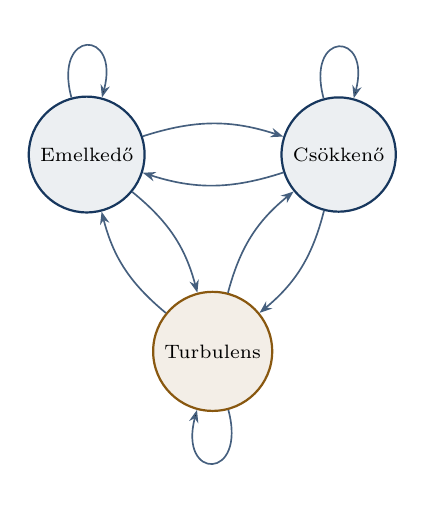
\begin{tikzpicture}[font=\scriptsize,
          st/.style={circle, draw=tdkblue, line width=.8pt, fill=tdkblue!8,
            minimum size=1.4cm, align=center},
          tr/.style={-{Stealth[length=1.6mm]}, draw=tdkblue!80, line width=.6pt}]
        \node[st] (up) at (0,0) {Emelkedő};
        \node[st] (down) at (3.2,0) {Csökkenő};
        \node[st, draw=eventochre, fill=eventochre!10] (turb) at (1.6,-2.5) {Turbulens};
        \draw[tr] (up) to[bend left=18] (down);
        \draw[tr] (down) to[bend left=18] (up);
        \draw[tr] (up) to[bend left=18] (turb);
        \draw[tr] (turb) to[bend left=18] (up);
        \draw[tr] (down) to[bend left=18] (turb);
        \draw[tr] (turb) to[bend left=18] (down);
        \draw[tr] (up) edge[loop above, looseness=6] (up);
        \draw[tr] (down) edge[loop above, looseness=6] (down);
        \draw[tr] (turb) edge[loop below, looseness=6] (turb);
      \end{tikzpicture}
      \par\smallskip{\scriptsize Nyilak: átmenet egyik napról a másikra ($A_{jk}$)}
    \end{column}
    \begin{column}{.53\textwidth}
      \small
      \textbf{Megfigyelés} $\mathbf{x}_t$: napi loghozam és EWMA-volatilitás
      (standardizálva).\par\smallskip
      \textbf{Frissítés napról napra}, csak a $t$. napig ismert adatból:
      \[
        p_t(k)\;\propto\;b_k(\mathbf{x}_t)\sum_{j=1}^{3}p_{t-1}(j)\,A_{jk}
      \]
      {\footnotesize $p_t(k)$: a $k$. állapot valószínűsége\\
      $b_k$: mennyire illik a mai megfigyelés az állapothoz\\
      $A_{jk}$: átmenet $j$-ből $k$-ba\par}
      \smallskip
      \begin{block}{Mi kerül a modellbe?}
        \small A 3 valószínűség, új jellemzőként. Illesztés csak a
        tanítószakaszon; a simított változat a jövőt is látná.
      \end{block}
    \end{column}
  \end{columns}
  % EM-illesztés (Baum-Welch), 300 iteráció, seed 42. Turbulens = a legnagyobb
  % szórású állapot, a másik kettő az átlagos hozam szerint.
\end{frame}

% 8 | 6:10--7:10
\begin{frame}{Kétlépcsős kapu: mikor váltja le a modell a referenciát?}
  \begin{columns}[T,onlytextwidth]
    \begin{column}{.48\textwidth}
      \begin{block}{1. Jobb-e a validáción?}
        \small
        Naponta összevetjük a jelöltek és a referencia hibáját.
        Hansen-féle SPA-próba az \textbf{összes} jelöltre egyszerre
        (több száz), 2000 blokkos újramintázással. Feltétel: $p<0{,}10$.
      \end{block}
    \end{column}
    \begin{column}{.48\textwidth}
      \begin{block}{2. Megismétlődik-e?}
        \small
        A győztest a tanítószakasz 4 elkülönített blokkján is ellenőrizzük;
        minden blokkra a többin tanult modell becsül. Feltétel: $p<0{,}10$;
        ingadozásnál $p<0{,}05$, HAR-tartalékkal.
      \end{block}
    \end{column}
  \end{columns}
  \medskip
  \begin{block}{Alapértelmezés}
    Ha bármelyik lépcső nem teljesül, a becslés a referencia:
    árnál az utolsó záróár, ingadozásnál az EWMA-variancia.
  \end{block}
  % Hiba: árnál abszolút százalékos hiba, ingadozásnál QLIKE.
\end{frame}

% 9 | 7:10--8:00
\begin{frame}{Miért ezek a módszerek?}
  \centering\small
  \renewcommand{\arraystretch}{1.25}
  \begin{tabular}{@{}L{.28\linewidth}L{.33\linewidth}L{.33\linewidth}@{}}
    \toprule
    \textbf{Probléma} & \textbf{Választott megoldás} & \textbf{Elvetett alternatíva}\\
    \midrule
    Jövőbeli adat szivárgása & időrendi felosztás, purge + embargó & kevert (véletlen) felosztás\\
    Sok jelöltből egy véletlenül jó & SPA az összes jelöltre & legjobb kiválasztása, páros DM-próba\\
    Időszakhoz kötött előny & ismétlődés a tanítóablakon belül & egyetlen validációs időszak\\
    Rezsim jövőbelátás nélkül & HMM forward-szűrés & simított HMM-valószínűség\\
    Kis, táblázatos adat & LightGBM & neurális hálók (V5--V7-ben gyengébbek)\\
    Zajos variancia-mérés & QLIKE (Patton 2011) & abszolút hiba\\
    \bottomrule
  \end{tabular}
  % A Python kézenfekvő eszközei (pl. kevert train_test_split, simított
  % predict_proba) itt jövőbeli információt csempésznének a modellbe.
\end{frame}

% 10 | 8:00--9:00
\begin{frame}{Első mérés és végleges futás: mit változtatott a kapu?}
  \framesubtitle{Egynapos ár \,·\, ugyanaz a 29 dátumpár $\times$ 50 seed \,·\, külső előrejelzések}
  \centering
  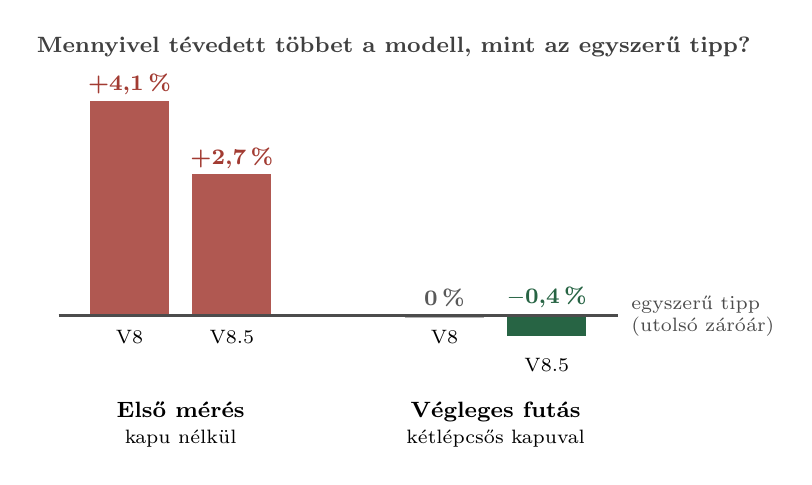
\begin{tikzpicture}[x=1cm, y=0.66cm, font=\small]
    % 0 = az egyszerű tipp hibája; felfelé: a modell többet tévedett
    \fill[lossred!85] (0.6,0) rectangle (1.6,4.14);
    \fill[lossred!85] (1.9,0) rectangle (2.9,2.72);
    \fill[black!30] (4.6,-0.04) rectangle (5.6,0.04);
    \fill[actualgreen] (5.9,0) rectangle (6.9,-0.39);
    \draw[black!70, line width=1pt] (0.2,0) -- (7.3,0);
    \node[anchor=west, font=\scriptsize, text=black!70, align=left] at (7.35,0)
      {egyszerű tipp\\(utolsó záróár)};
    \node[font=\footnotesize\bfseries, text=lossred] at (1.1,4.45) {+4,1\,\%};
    \node[font=\footnotesize\bfseries, text=lossred] at (2.4,3.03) {+2,7\,\%};
    \node[font=\footnotesize\bfseries, text=black!65] at (5.1,0.35) {0\,\%};
    \node[font=\footnotesize\bfseries, text=actualgreen] at (6.4,0.35) {$-$0,4\,\%};
    \node[font=\scriptsize] at (1.1,-0.4) {V8};
    \node[font=\scriptsize] at (2.4,-0.4) {V8.5};
    \node[font=\scriptsize] at (5.1,-0.4) {V8};
    \node[font=\scriptsize] at (6.4,-0.95) {V8.5};
    \node[font=\footnotesize, align=center] at (1.75,-2.1) {\textbf{Első mérés}\\ \scriptsize kapu nélkül};
    \node[font=\footnotesize, align=center] at (5.75,-2.1) {\textbf{Végleges futás}\\ \scriptsize kétlépcsős kapuval};
    \node[anchor=south west, font=\footnotesize\bfseries, text=black!75] at (-0.2,4.8)
      {Mennyivel tévedett többet a modell, mint az egyszerű tipp?};
  \end{tikzpicture}
  \par\smallskip\raggedright\small
  Kapu nélkül a modell átlagosan 3--4\,\%-kal nagyobbat tévedett, mint ha
  egyszerűen az utolsó záróárat mondtuk volna. A kapu után ugyanannyit vagy
  kicsit kevesebbet téved.
  % Átlagos hiba (MAPE): egyszerű tipp 2,54%; első mérés V8 2,64%, V8.5 2,61%;
  % végleges V8 2,54%, V8.5 2,53%. Relatív eltérés = (modell - tipp) / tipp.
  % Első mérésben a futások 47% / 46%-ában volt jobb a modell, a többiben rosszabb.
  % A 6. pár az első mérésben HMM-hibával elmaradt, ezért a közös 29 páron vetjük össze.
  % Forrás: data/repeated_experiment/main.xlsx és V8_V85_osszehasonlitas.xlsx.
\end{frame}

% 11 | 9:00--10:10
\begin{frame}{Ki volt pontosabb: a modell vagy az egyszerű tipp?}
  \framesubtitle{18\,000 előrejelzés \,·\, egyszerű tipp: az ár ugyanannyi marad, az ingadozás a megszokott}
  \centering
  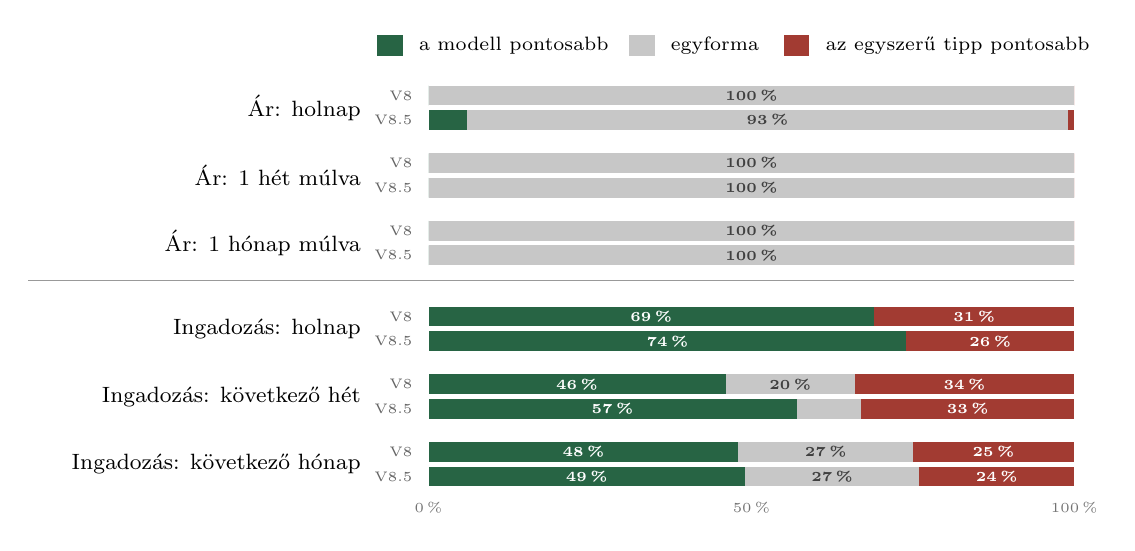
\begin{tikzpicture}[x=0.82mm, y=0.78mm, font=\scriptsize]
    \qmbar{58}{V8}{0}{100}{0}   \qmbar{54}{V8.5}{6}{93}{1}
    \qmbar{47}{V8}{0}{100}{0}   \qmbar{43}{V8.5}{0}{100}{0}
    \qmbar{36}{V8}{0}{100}{0}   \qmbar{32}{V8.5}{0}{100}{0}
    \qmbar{22}{V8}{69}{0}{31}   \qmbar{18}{V8.5}{74}{0}{26}
    \qmbar{11}{V8}{46}{20}{34}  \qmbar{7}{V8.5}{57}{10}{33}
    \qmbar{0}{V8}{48}{27}{25}   \qmbar{-4}{V8.5}{49}{27}{24}
    \foreach \y/\t in {57.6/{Ár: holnap}, 46.6/{Ár: 1 hét múlva}, 35.6/{Ár: 1 hónap múlva},
        21.6/{Ingadozás: holnap}, 10.6/{Ingadozás: következő hét}, -0.4/{Ingadozás: következő hónap}}
      \node[anchor=east, font=\footnotesize] at (-9,\y) {\t};
    \draw[black!40] (-62,29.5) -- (100,29.5);
    \foreach \x in {0,50,100} \node[text=black!55, font=\tiny] at (\x,-7.5) {\x\,\%};
    % jelmagyarázat
    \fill[actualgreen] (-8,66) rectangle (-4,69.5); \node[anchor=west] at (-3,67.75) {a modell pontosabb};
    \fill[black!22] (31,66) rectangle (35,69.5); \node[anchor=west] at (36,67.75) {egyforma};
    \fill[lossred] (55,66) rectangle (59,69.5); \node[anchor=west] at (60,67.75) {az egyszerű tipp pontosabb};
  \end{tikzpicture}
  % Áron a kapu szinte mindig az egyszerű tippet hagyta meg (szürke = egyforma).
  % Ingadozásban holnapra 69-74%-ban a modell volt pontosabb.
\end{frame}

% 12 | 10:10--11:10
\begin{frame}{Ingadozás holnapra: becslés és valóság}
  \framesubtitle{V8.5, a 30 külső célnap \,·\, a modell az 50 seed átlaga \,·\, napi volatilitás (\%)}
  \centering
  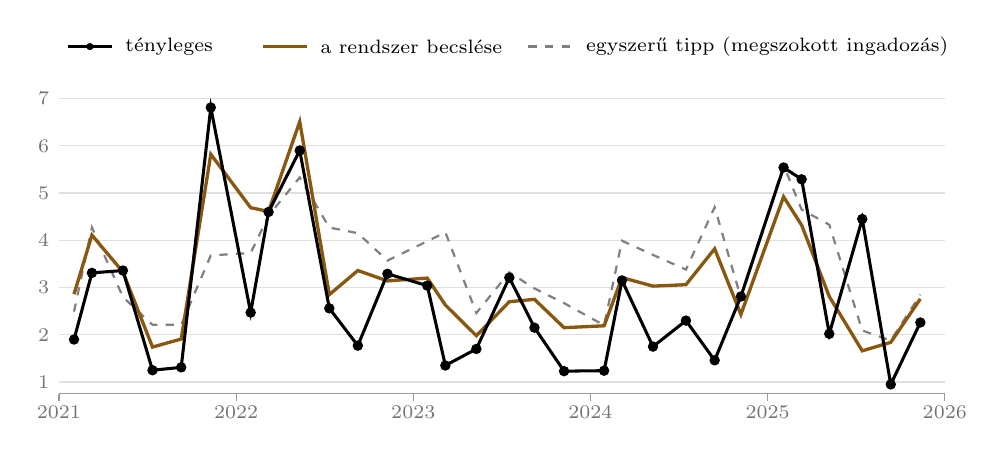
\begin{tikzpicture}[x=2.25cm, y=0.6cm, font=\scriptsize]
    \foreach \v in {1,...,7} {
      \draw[black!12] (0,\v) -- (5,\v);
      \node[anchor=east, text=black!55] at (0,\v) {\v};
    }
    \foreach \t in {0,...,5} {
      \draw[black!40] (\t,0.6) -- (\t,0.75);
      \pgfmathtruncatemacro{\yr}{2021+\t}
      \node[text=black!55] at (\t,0.35) {\yr};
    }
    \draw[black!40] (0,0.75) -- (5,0.75);
    \draw[black!50, dashed, line width=.8pt] plot coordinates {(0.085,2.49) (0.186,4.27) (0.361,2.80) (0.528,2.21) (0.690,2.21) (0.857,3.68) (1.082,3.73) (1.183,4.52) (1.359,5.33) (1.526,4.27) (1.687,4.15) (1.854,3.57) (2.079,3.98) (2.181,4.17) (2.356,2.46) (2.542,3.32) (2.684,2.98) (2.851,2.67) (3.077,2.20) (3.178,3.99) (3.353,3.69) (3.539,3.38) (3.701,4.70) (3.849,2.78) (4.090,5.59) (4.192,4.65) (4.348,4.33) (4.534,2.09) (4.695,1.88) (4.862,2.85)};
    \draw[eventochre, line width=1.2pt] plot coordinates {(0.085,2.86) (0.186,4.11) (0.361,3.33) (0.528,1.74) (0.690,1.91) (0.857,5.82) (1.082,4.69) (1.183,4.61) (1.359,6.51) (1.526,2.85) (1.687,3.36) (1.854,3.14) (2.079,3.20) (2.181,2.63) (2.356,1.98) (2.542,2.70) (2.684,2.75) (2.851,2.15) (3.077,2.19) (3.178,3.21) (3.353,3.03) (3.539,3.06) (3.701,3.82) (3.849,2.43) (4.090,4.92) (4.192,4.32) (4.348,2.81) (4.534,1.66) (4.695,1.84) (4.862,2.76)};
    \draw[black, line width=1.1pt] plot[mark=*, mark size=1.3pt] coordinates {(0.085,1.90) (0.186,3.31) (0.361,3.36) (0.528,1.25) (0.690,1.31) (0.857,6.81) (1.082,2.47) (1.183,4.60) (1.359,5.90) (1.526,2.56) (1.687,1.77) (1.854,3.29) (2.079,3.04) (2.181,1.35) (2.356,1.70) (2.542,3.21) (2.684,2.15) (2.851,1.23) (3.077,1.24) (3.178,3.15) (3.353,1.75) (3.539,2.30) (3.701,1.46) (3.849,2.81) (4.090,5.54) (4.192,5.29) (4.348,2.02) (4.534,4.45) (4.695,0.95) (4.862,2.26)};
    % jelmagyarázat
    \draw[black, line width=1.1pt] (0.05,8.1) -- (0.3,8.1); \fill (0.175,8.1) circle (1.3pt);
    \node[anchor=west] at (0.32,8.1) {tényleges};
    \draw[eventochre, line width=1.2pt] (1.15,8.1) -- (1.4,8.1);
    \node[anchor=west] at (1.42,8.1) {a rendszer becslése};
    \draw[black!50, dashed, line width=.8pt] (2.65,8.1) -- (2.9,8.1);
    \node[anchor=west] at (2.92,8.1) {egyszerű tipp (megszokott ingadozás)};
  \end{tikzpicture}
  \par\smallskip\raggedright\small
  A 30 célnapból \textbf{22-n} a rendszer becslése volt közelebb a tényleges
  ingadozáshoz; átlagos hiba 1,06 vs.\ 1,48 százalékpont.
  Ár: a rendszer mindhárom távon az egyszerű tippet adja (hiba 2,58\,/\,5,19\,/\,9,54\,\%).
  % Közelebb = kisebb abszolút eltérés a volatilitás-százalékban. A kiválasztás QLIKE-kal
  % történt; QLIKE szerint 23/30 célnapon jobb a modell. 2025 júliusában (28. pár) a
  % hirtelen ugrást egyik becslés sem látta előre. Csak 30 célnap: nem szignifikáns.
\end{frame}

% 13 | 11:10--13:00
\section{Összefoglalás}
\begin{frame}{Összefoglalás}
  \begin{columns}[T,onlytextwidth]
    \begin{column}{.48\textwidth}
      \begin{block}{Ár}
        Szigorú kiválasztás mellett az utolsó záróár nem győzhető le
        egyik távon sem; több adatfajta (V8) és több minta (V8.5) sem segít.
      \end{block}
    \end{column}
    \begin{column}{.48\textwidth}
      \begin{block}{Ingadozás}
        A modell átlagosan jobb az EWMA-nál, legerősebben egynapos távon;
        a különbség még nem szignifikáns.
      \end{block}
    \end{column}
  \end{columns}
  \medskip
  \textbf{Hozzájárulás:} reprodukálható, szivárgásmentes kísérleti keret,
  amely a negatív eredményt is kimutatja.\par\medskip
  \textbf{Következő lépés:} új, 2025-11-12 utáni lezárásokon, érintetlen
  adaton ellenőrizni az ingadozás-előnyt.
  \par\bigskip\centering\textbf{Köszönöm a figyelmet!}
\end{frame}

% =====================================================================
\appendix
\begingroup
\setbeamertemplate{footline}{}

\begin{frame}[noframenumbering]{Tartalék · A hibakülönbség eloszlása dátumpáronként}
  \centering
  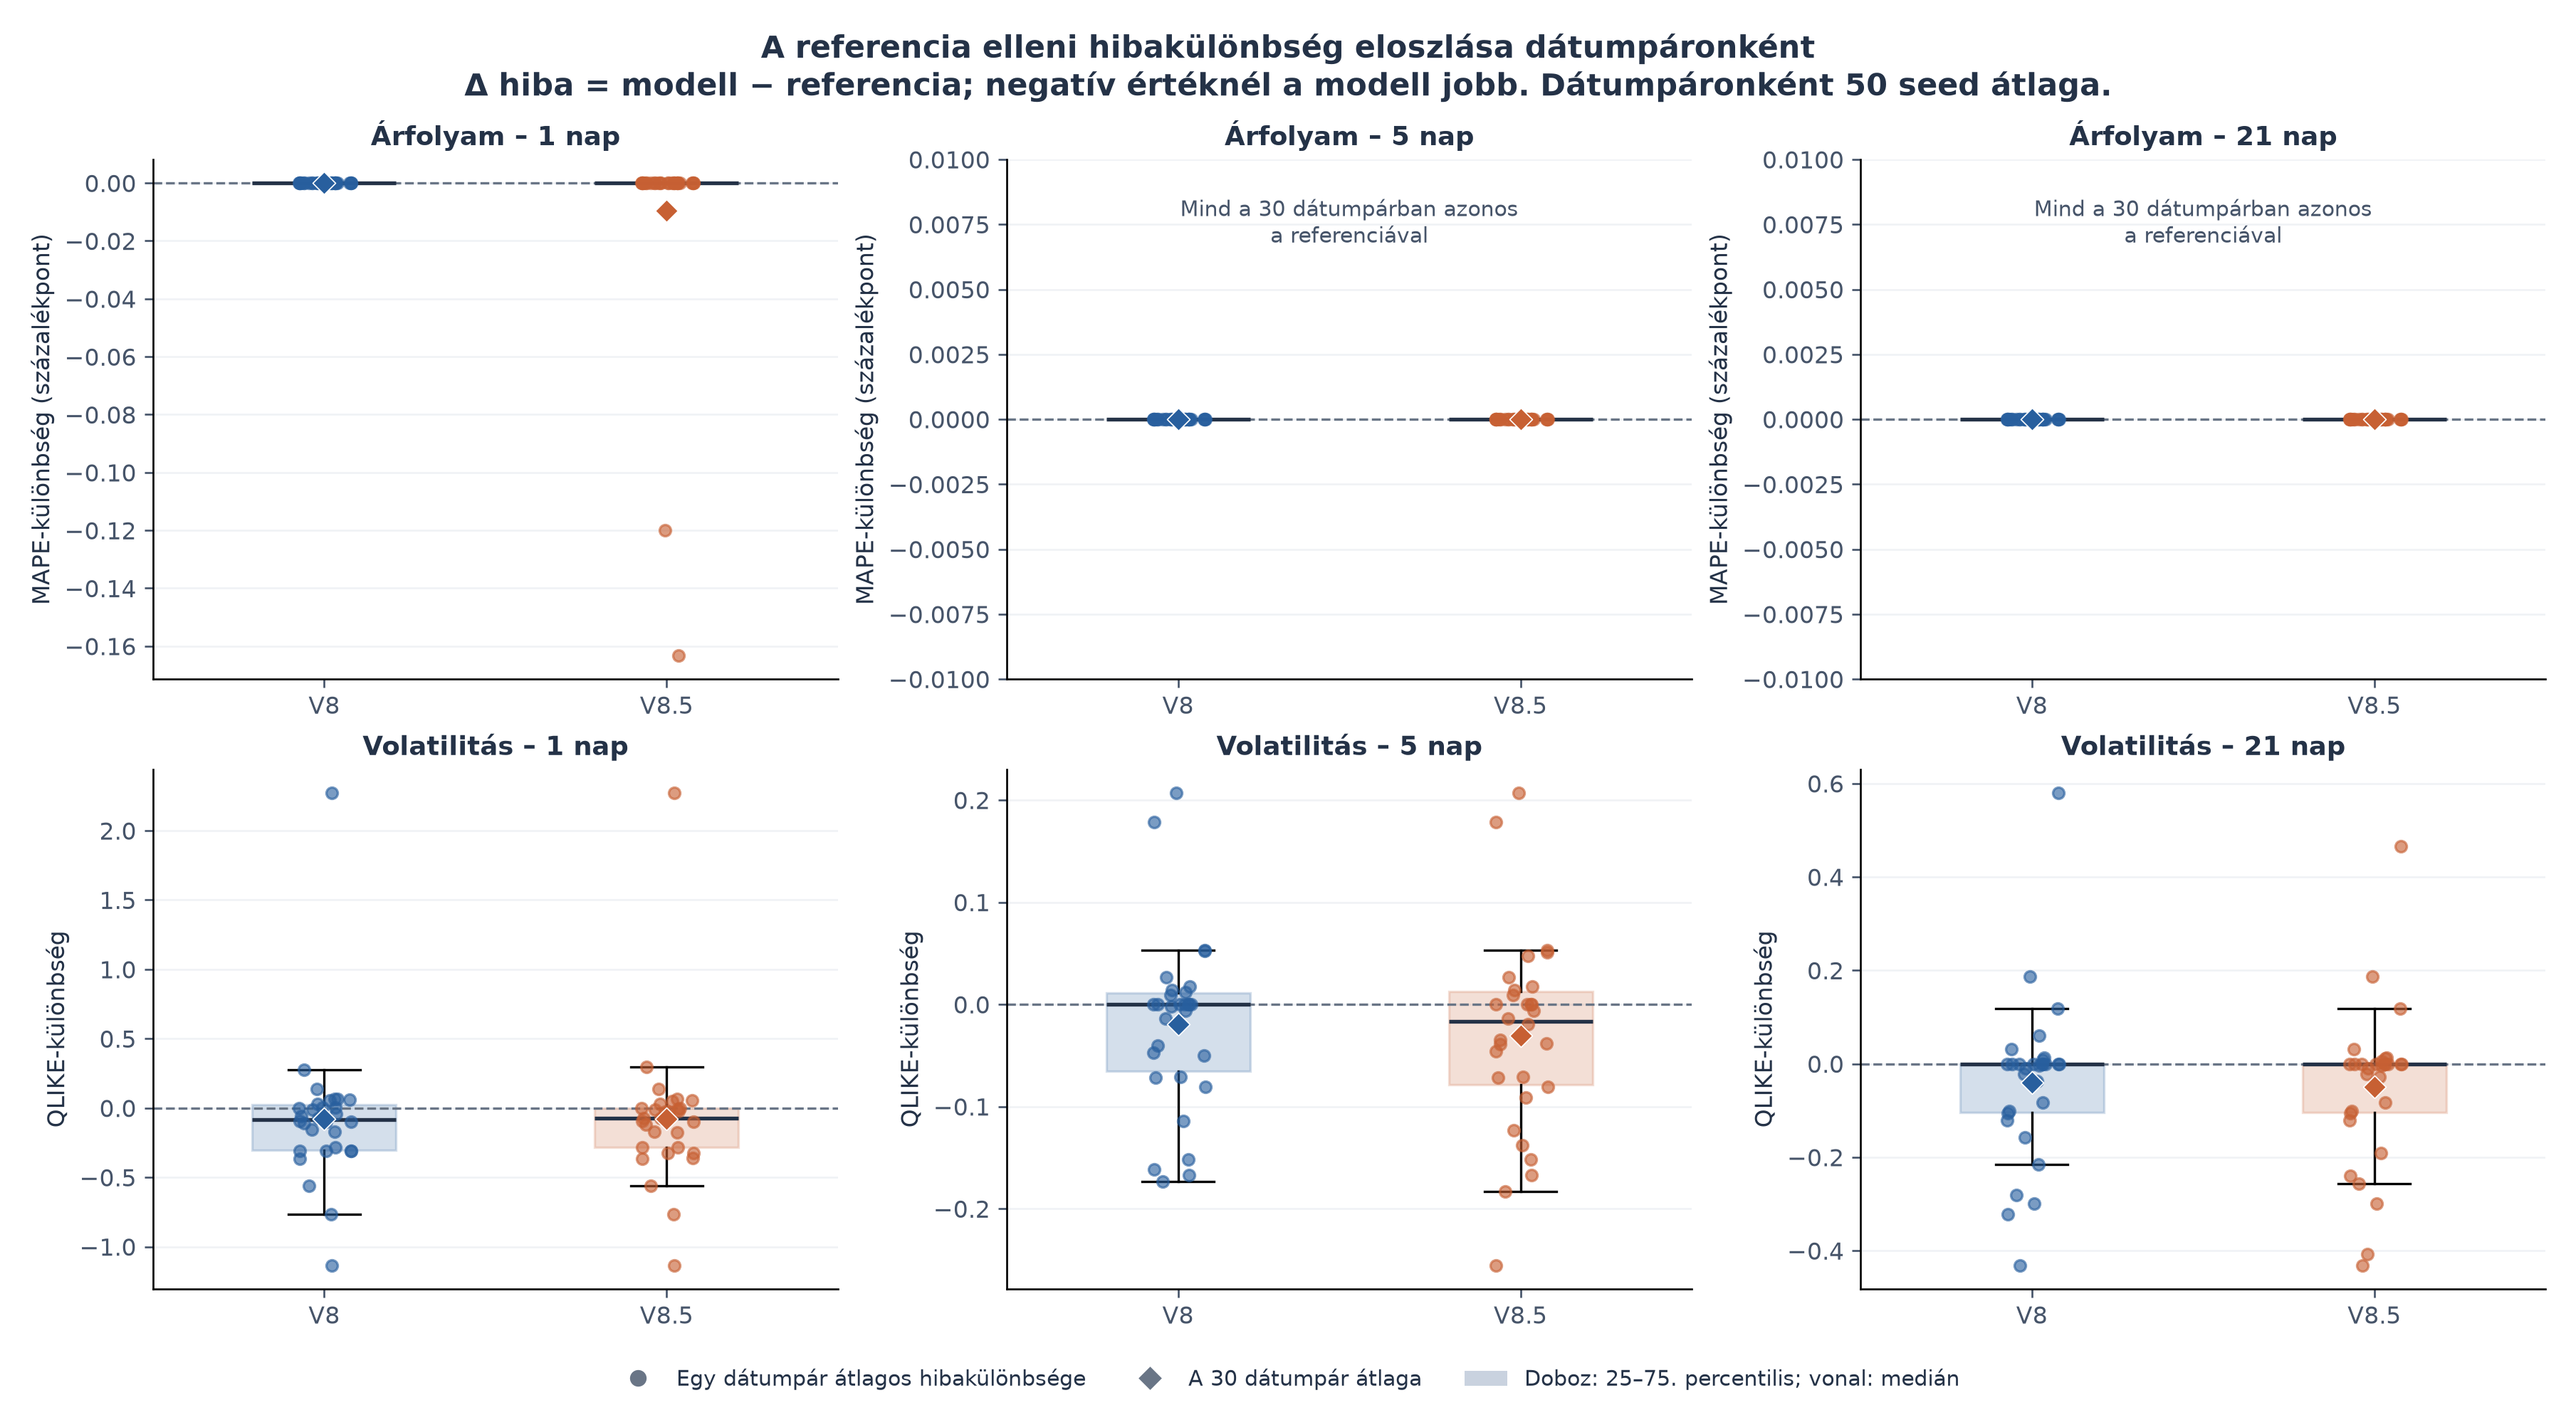
\includegraphics[width=\textwidth,height=.82\textheight,keepaspectratio]{abra_hibakulonbseg.png}
\end{frame}

\begin{frame}[noframenumbering]{Tartalék · Korlátok}
  \centering\small
  \renewcommand{\arraystretch}{1.25}
  \begin{tabular}{@{}L{.4\linewidth}L{.54\linewidth}@{}}
    \toprule
    \textbf{Korlát} & \textbf{Következmény}\\
    \midrule
    30 célnap sávonként & az intervallumok érintik a nullát\\
    A 2.\ és 3.\ protokoll az első mérés után készült & a tesztablakok nem érintetlenek; új lezárások kellenek\\
    Egyetlen részvény (NVIDIA) & az általánosíthatóság nem igazolt\\
    Pooled univerzum: ma is létező cégek & túlélési torzítás lehetséges\\
    60 perces adat csak kb. 2 év & az intraday réteg nem versenyzett\\
    Nincs tranzakciós költség & kereskedési haszon nem állítható\\
    \bottomrule
  \end{tabular}
\end{frame}
\endgroup

\end{document}
